\section{Performance of similar tools}
Other tools that are easy to find and rather easy to use tend to estimate
power on a lower abstraction level than PET, thus it is natural that they
require more knowledge about implementation, but will also give you a more
trustworthy estimate. Never the less, it seems that PET is not very far off,
given its results compared to the similar tools.

\subsection{McPAT}

\begin{figure}[htb]
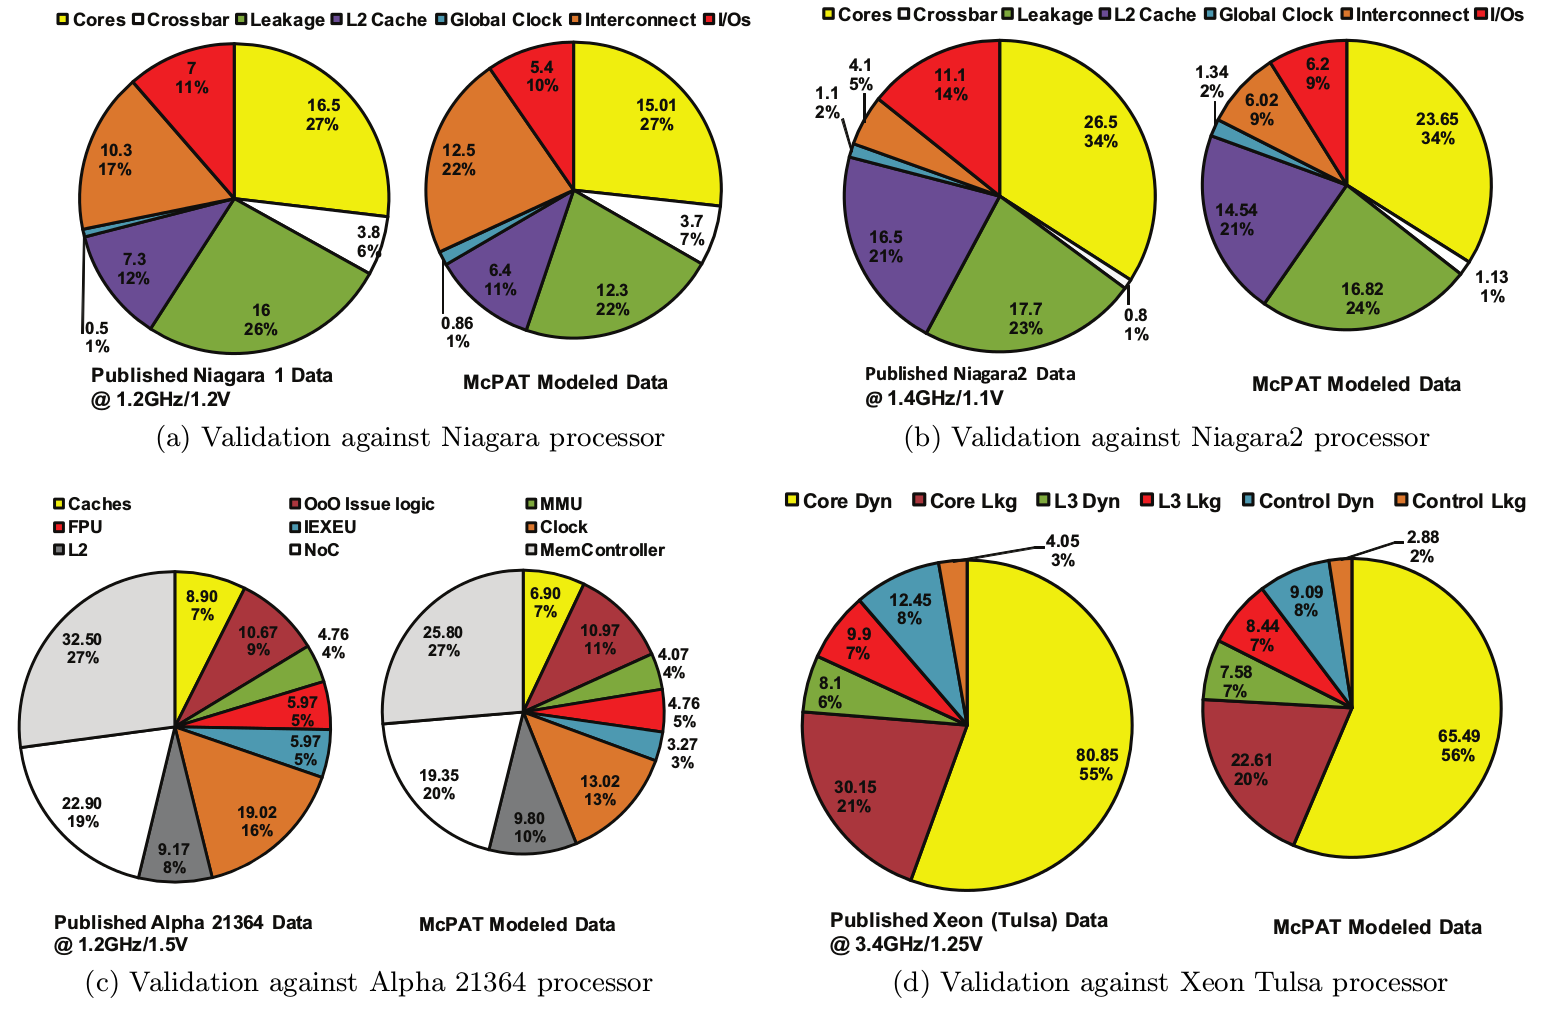
\includegraphics[width=\textwidth]{figs/mcpat-performance.png}
\caption{McPAT performance, borrowed from Figure 3 in \cite{li2009mcpat}}
\label{fig:mcpat-perf}
\end{figure}

From the McPAT paper \cite{li2009mcpat} and \autoref{fig:mcpat-perf} it is
stated that McPAT managed model an Alpha 21364 core within 2.78\% error, and is
in general between 10\% and 20\% off. McPAT does also predict area and timings,
but does also require a quite extensive XML-file with over 250 parameters.

\subsection{Wattch}

Wattch connects with SimpleScalar and uses live data and capacitance models to
estimate power. \cite{brooks2000wattch} states that the models are generally
within 10\% of real power consumption, and that the power breakdown models are
generally within 13.3\%. It should be mentioned that Wattch depends on
transistor scaling for it's models to work correctly, and after the end of
Dennard-scaling, the equations does no longer apply to modern process
technologies.


